% Options for packages loaded elsewhere
\PassOptionsToPackage{unicode}{hyperref}
\PassOptionsToPackage{hyphens}{url}
\PassOptionsToPackage{dvipsnames,svgnames,x11names}{xcolor}
%
\documentclass[
  letterpaper,
  DIV=11,
  numbers=noendperiod]{scrartcl}

\usepackage{amsmath,amssymb}
\usepackage{iftex}
\ifPDFTeX
  \usepackage[T1]{fontenc}
  \usepackage[utf8]{inputenc}
  \usepackage{textcomp} % provide euro and other symbols
\else % if luatex or xetex
  \usepackage{unicode-math}
  \defaultfontfeatures{Scale=MatchLowercase}
  \defaultfontfeatures[\rmfamily]{Ligatures=TeX,Scale=1}
\fi
\usepackage{lmodern}
\ifPDFTeX\else  
    % xetex/luatex font selection
\fi
% Use upquote if available, for straight quotes in verbatim environments
\IfFileExists{upquote.sty}{\usepackage{upquote}}{}
\IfFileExists{microtype.sty}{% use microtype if available
  \usepackage[]{microtype}
  \UseMicrotypeSet[protrusion]{basicmath} % disable protrusion for tt fonts
}{}
\makeatletter
\@ifundefined{KOMAClassName}{% if non-KOMA class
  \IfFileExists{parskip.sty}{%
    \usepackage{parskip}
  }{% else
    \setlength{\parindent}{0pt}
    \setlength{\parskip}{6pt plus 2pt minus 1pt}}
}{% if KOMA class
  \KOMAoptions{parskip=half}}
\makeatother
\usepackage{xcolor}
\setlength{\emergencystretch}{3em} % prevent overfull lines
\setcounter{secnumdepth}{2}
% Make \paragraph and \subparagraph free-standing
\ifx\paragraph\undefined\else
  \let\oldparagraph\paragraph
  \renewcommand{\paragraph}[1]{\oldparagraph{#1}\mbox{}}
\fi
\ifx\subparagraph\undefined\else
  \let\oldsubparagraph\subparagraph
  \renewcommand{\subparagraph}[1]{\oldsubparagraph{#1}\mbox{}}
\fi

\usepackage{color}
\usepackage{fancyvrb}
\newcommand{\VerbBar}{|}
\newcommand{\VERB}{\Verb[commandchars=\\\{\}]}
\DefineVerbatimEnvironment{Highlighting}{Verbatim}{commandchars=\\\{\}}
% Add ',fontsize=\small' for more characters per line
\usepackage{framed}
\definecolor{shadecolor}{RGB}{241,243,245}
\newenvironment{Shaded}{\begin{snugshade}}{\end{snugshade}}
\newcommand{\AlertTok}[1]{\textcolor[rgb]{0.68,0.00,0.00}{#1}}
\newcommand{\AnnotationTok}[1]{\textcolor[rgb]{0.37,0.37,0.37}{#1}}
\newcommand{\AttributeTok}[1]{\textcolor[rgb]{0.40,0.45,0.13}{#1}}
\newcommand{\BaseNTok}[1]{\textcolor[rgb]{0.68,0.00,0.00}{#1}}
\newcommand{\BuiltInTok}[1]{\textcolor[rgb]{0.00,0.23,0.31}{#1}}
\newcommand{\CharTok}[1]{\textcolor[rgb]{0.13,0.47,0.30}{#1}}
\newcommand{\CommentTok}[1]{\textcolor[rgb]{0.37,0.37,0.37}{#1}}
\newcommand{\CommentVarTok}[1]{\textcolor[rgb]{0.37,0.37,0.37}{\textit{#1}}}
\newcommand{\ConstantTok}[1]{\textcolor[rgb]{0.56,0.35,0.01}{#1}}
\newcommand{\ControlFlowTok}[1]{\textcolor[rgb]{0.00,0.23,0.31}{#1}}
\newcommand{\DataTypeTok}[1]{\textcolor[rgb]{0.68,0.00,0.00}{#1}}
\newcommand{\DecValTok}[1]{\textcolor[rgb]{0.68,0.00,0.00}{#1}}
\newcommand{\DocumentationTok}[1]{\textcolor[rgb]{0.37,0.37,0.37}{\textit{#1}}}
\newcommand{\ErrorTok}[1]{\textcolor[rgb]{0.68,0.00,0.00}{#1}}
\newcommand{\ExtensionTok}[1]{\textcolor[rgb]{0.00,0.23,0.31}{#1}}
\newcommand{\FloatTok}[1]{\textcolor[rgb]{0.68,0.00,0.00}{#1}}
\newcommand{\FunctionTok}[1]{\textcolor[rgb]{0.28,0.35,0.67}{#1}}
\newcommand{\ImportTok}[1]{\textcolor[rgb]{0.00,0.46,0.62}{#1}}
\newcommand{\InformationTok}[1]{\textcolor[rgb]{0.37,0.37,0.37}{#1}}
\newcommand{\KeywordTok}[1]{\textcolor[rgb]{0.00,0.23,0.31}{#1}}
\newcommand{\NormalTok}[1]{\textcolor[rgb]{0.00,0.23,0.31}{#1}}
\newcommand{\OperatorTok}[1]{\textcolor[rgb]{0.37,0.37,0.37}{#1}}
\newcommand{\OtherTok}[1]{\textcolor[rgb]{0.00,0.23,0.31}{#1}}
\newcommand{\PreprocessorTok}[1]{\textcolor[rgb]{0.68,0.00,0.00}{#1}}
\newcommand{\RegionMarkerTok}[1]{\textcolor[rgb]{0.00,0.23,0.31}{#1}}
\newcommand{\SpecialCharTok}[1]{\textcolor[rgb]{0.37,0.37,0.37}{#1}}
\newcommand{\SpecialStringTok}[1]{\textcolor[rgb]{0.13,0.47,0.30}{#1}}
\newcommand{\StringTok}[1]{\textcolor[rgb]{0.13,0.47,0.30}{#1}}
\newcommand{\VariableTok}[1]{\textcolor[rgb]{0.07,0.07,0.07}{#1}}
\newcommand{\VerbatimStringTok}[1]{\textcolor[rgb]{0.13,0.47,0.30}{#1}}
\newcommand{\WarningTok}[1]{\textcolor[rgb]{0.37,0.37,0.37}{\textit{#1}}}

\providecommand{\tightlist}{%
  \setlength{\itemsep}{0pt}\setlength{\parskip}{0pt}}\usepackage{longtable,booktabs,array}
\usepackage{calc} % for calculating minipage widths
% Correct order of tables after \paragraph or \subparagraph
\usepackage{etoolbox}
\makeatletter
\patchcmd\longtable{\par}{\if@noskipsec\mbox{}\fi\par}{}{}
\makeatother
% Allow footnotes in longtable head/foot
\IfFileExists{footnotehyper.sty}{\usepackage{footnotehyper}}{\usepackage{footnote}}
\makesavenoteenv{longtable}
\usepackage{graphicx}
\makeatletter
\def\maxwidth{\ifdim\Gin@nat@width>\linewidth\linewidth\else\Gin@nat@width\fi}
\def\maxheight{\ifdim\Gin@nat@height>\textheight\textheight\else\Gin@nat@height\fi}
\makeatother
% Scale images if necessary, so that they will not overflow the page
% margins by default, and it is still possible to overwrite the defaults
% using explicit options in \includegraphics[width, height, ...]{}
\setkeys{Gin}{width=\maxwidth,height=\maxheight,keepaspectratio}
% Set default figure placement to htbp
\makeatletter
\def\fps@figure{htbp}
\makeatother

\KOMAoption{captions}{tableheading}
\usepackage{marginnote, here, relsize, needspace, setspace} \def\it{\emph}
\makeatletter
\@ifpackageloaded{caption}{}{\usepackage{caption}}
\AtBeginDocument{%
\ifdefined\contentsname
  \renewcommand*\contentsname{Table of contents}
\else
  \newcommand\contentsname{Table of contents}
\fi
\ifdefined\listfigurename
  \renewcommand*\listfigurename{List of Figures}
\else
  \newcommand\listfigurename{List of Figures}
\fi
\ifdefined\listtablename
  \renewcommand*\listtablename{List of Tables}
\else
  \newcommand\listtablename{List of Tables}
\fi
\ifdefined\figurename
  \renewcommand*\figurename{Figure}
\else
  \newcommand\figurename{Figure}
\fi
\ifdefined\tablename
  \renewcommand*\tablename{Table}
\else
  \newcommand\tablename{Table}
\fi
}
\@ifpackageloaded{float}{}{\usepackage{float}}
\floatstyle{ruled}
\@ifundefined{c@chapter}{\newfloat{codelisting}{h}{lop}}{\newfloat{codelisting}{h}{lop}[chapter]}
\floatname{codelisting}{Listing}
\newcommand*\listoflistings{\listof{codelisting}{List of Listings}}
\makeatother
\makeatletter
\makeatother
\makeatletter
\@ifpackageloaded{caption}{}{\usepackage{caption}}
\@ifpackageloaded{subcaption}{}{\usepackage{subcaption}}
\makeatother
\ifLuaTeX
  \usepackage{selnolig}  % disable illegal ligatures
\fi
\usepackage{bookmark}

\IfFileExists{xurl.sty}{\usepackage{xurl}}{} % add URL line breaks if available
\urlstyle{same} % disable monospaced font for URLs
\hypersetup{
  pdftitle={Lab 4 - Multinomial Regression - Questions},
  pdfauthor={Suyog Chandramouli},
  colorlinks=true,
  linkcolor={blue},
  filecolor={Maroon},
  citecolor={Blue},
  urlcolor={Blue},
  pdfcreator={LaTeX via pandoc}}

\title{Lab 4 - Multinomial Regression - Questions}
\author{Suyog Chandramouli}
\date{2025-02-26}

\begin{document}
\maketitle

Lab Goal: Predict voting frequency using demographic variables Data
source: FiveThirtyEight ``Why Many Americans Don't Vote'' survey Method:
Multinomial logistic regression

\subsection{Data}\label{data}

The data for this assignment comes from an online Ipsos survey that was
conducted for the FiveThirtyEight article
\href{https://projects.fivethirtyeight.com/non-voters-poll-2020-election/}{``Why
Many Americans Don't Vote''}. You can read more about the survey design
and respondents in the README of the
\href{https://github.com/fivethirtyeight/data/tree/master/non-voters}{GitHub
repo} for the data.

Respondents were asked a variety of questions about their political
beliefs, thoughts on multiple issues, and voting behavior. We will focus
on using the demographic variables and someone's party identification to
understand whether a person is a probable voter.

The variables we'll focus on were (definitions from the codebook in data
set GitHub repo):

\begin{itemize}
\item
  \texttt{ppage}: Age of respondent
\item
  \texttt{educ}: Highest educational attainment category.\\
\item
  \texttt{race}: Race of respondent, census categories. Note: all
  categories except Hispanic were non-Hispanic.
\item
  \texttt{gender}: Gender of respondent
\item
  \texttt{income\_cat}: Household income category of respondent
\item
  \texttt{Q30}: Response to the question ``Generally speaking, do you
  think of yourself as a\ldots{}''

  \begin{itemize}
  \tightlist
  \item
    1: Republican
  \item
    2: Democrat
  \item
    3: Independent
  \item
    4: Another party, please specify
  \item
    5: No preference
  \item
    -1: No response
  \end{itemize}
\item
  \texttt{voter\_category}: past voting behavior:

  \begin{itemize}
  \tightlist
  \item
    \textbf{always}: respondent voted in all or all-but-one of the
    elections they were eligible in
  \item
    \textbf{sporadic}: respondent voted in at least two, but fewer than
    all-but-one of the elections they were eligible in
  \item
    \textbf{rarely/never}: respondent voted in 0 or 1 of the elections
    they were eligible in
  \end{itemize}
\end{itemize}

You can read in the data directly from the GitHub repo:

\begin{Shaded}
\begin{Highlighting}[]
\FunctionTok{library}\NormalTok{(nnet)}
\FunctionTok{library}\NormalTok{(car)}
\FunctionTok{library}\NormalTok{(tidyverse)}
\FunctionTok{library}\NormalTok{(emmeans)}
\FunctionTok{library}\NormalTok{(ggeffects)}
\FunctionTok{library}\NormalTok{(knitr)}
\FunctionTok{library}\NormalTok{(patchwork)}
\FunctionTok{library}\NormalTok{(broom)}
\FunctionTok{library}\NormalTok{(parameters)}
\FunctionTok{library}\NormalTok{(easystats)}
\end{Highlighting}
\end{Shaded}

\begin{Shaded}
\begin{Highlighting}[]
\NormalTok{voter\_data }\OtherTok{\textless{}{-}} \FunctionTok{read\_csv}\NormalTok{(}\StringTok{"https://raw.githubusercontent.com/fivethirtyeight/data/master/non{-}voters/nonvoters\_data.csv"}\NormalTok{)}
\end{Highlighting}
\end{Shaded}

\section{Lab}\label{lab}

\begin{itemize}
\tightlist
\item
  The variable \texttt{Q30} contains the respondent's political party
  identification. Make a new variable that simplifies \texttt{Q30} into
  four categories: ``Democrat'', ``Republican'', ``Independent'',
  ``Other'' (``Other'' also includes respondents who did not answer the
  question).
\end{itemize}

\begin{Shaded}
\begin{Highlighting}[]
\NormalTok{voter\_data }\OtherTok{\textless{}{-}}\NormalTok{ voter\_data }\SpecialCharTok{\%\textgreater{}\%}
  \FunctionTok{mutate}\NormalTok{(}\AttributeTok{pol\_ident\_new =} \FunctionTok{case\_when}\NormalTok{(}
\NormalTok{    Q30}\SpecialCharTok{==}\DecValTok{1} \SpecialCharTok{\textasciitilde{}} \StringTok{"Rep"}\NormalTok{, }
\NormalTok{    Q30}\SpecialCharTok{==}\DecValTok{2} \SpecialCharTok{\textasciitilde{}} \StringTok{"Dem"}\NormalTok{, }
\NormalTok{    Q30}\SpecialCharTok{==}\DecValTok{3} \SpecialCharTok{\textasciitilde{}} \StringTok{"Indep"}\NormalTok{, }
    \ConstantTok{TRUE} \SpecialCharTok{\textasciitilde{}} \StringTok{"Other"}
\NormalTok{  ))}
\end{Highlighting}
\end{Shaded}

\begin{itemize}
\tightlist
\item
  The variable \texttt{voter\_category} identifies the respondent's past
  voter behavior. Relevel the variable to make rarely/never the baseline
  level, followed by sporadic, then always
\end{itemize}

\begin{Shaded}
\begin{Highlighting}[]
\CommentTok{\#Enter your code}
\CommentTok{\# Figuring out what unique variables are available}
\FunctionTok{levels}\NormalTok{(}\FunctionTok{as.factor}\NormalTok{(voter\_data}\SpecialCharTok{$}\NormalTok{voter\_category))}
\end{Highlighting}
\end{Shaded}

\begin{verbatim}
[1] "always"       "rarely/never" "sporadic"    
\end{verbatim}

\begin{Shaded}
\begin{Highlighting}[]
\CommentTok{\# Reordering}
\NormalTok{voter\_data}\SpecialCharTok{$}\NormalTok{voter\_category }\OtherTok{=} \FunctionTok{relevel}\NormalTok{(}\FunctionTok{as.factor}\NormalTok{(voter\_data}\SpecialCharTok{$}\NormalTok{voter\_category), }\AttributeTok{ref =} \StringTok{"sporadic"}\NormalTok{)}

\CommentTok{\# Recheck level order}
\FunctionTok{levels}\NormalTok{(}\FunctionTok{as.factor}\NormalTok{(voter\_data}\SpecialCharTok{$}\NormalTok{voter\_category))}
\end{Highlighting}
\end{Shaded}

\begin{verbatim}
[1] "sporadic"     "always"       "rarely/never"
\end{verbatim}

\begin{itemize}
\tightlist
\item
  Center the age variable to make the intercept more interepretable.
  That is, so that it reflects the log-odds for an average-aged person
  rather than a 0-year old person
\end{itemize}

\begin{Shaded}
\begin{Highlighting}[]
\CommentTok{\# enter code }

\NormalTok{voter\_data}\OtherTok{=}\NormalTok{voter\_data }\SpecialCharTok{\%\textgreater{}\%}
  \FunctionTok{mutate}\NormalTok{(}\AttributeTok{ppage\_centered =}\NormalTok{ ppage }\SpecialCharTok{{-}} \FunctionTok{mean}\NormalTok{(ppage))}
\end{Highlighting}
\end{Shaded}

\begin{itemize}
\tightlist
\item
  In the
  \href{https://projects.fivethirtyeight.com/non-voters-poll-2020-election/}{FiveThirtyEight
  article}, the authors include visualizations of the relationship
  between the voter category and demographic variables such as race,
  age, education, etc. Select two demographic variables. For each
  variable, try to replicate the visualizations and interpret the plot
  to describe its relationship with voter category. Have fun with it:
  https://www.mikelee.co/posts/2020-02-08-recreate-fivethirtyeight-chicklet-stacked-bar-chart-in-ggplot2.
\end{itemize}

\begin{Shaded}
\begin{Highlighting}[]
\CommentTok{\# library}
\FunctionTok{library}\NormalTok{(ggplot2)}
\FunctionTok{library}\NormalTok{(viridis)}
\FunctionTok{library}\NormalTok{(cowplot)}

\CommentTok{\# Enter code}
\NormalTok{plot1}\OtherTok{=}\FunctionTok{ggplot}\NormalTok{(voter\_data, }\FunctionTok{aes}\NormalTok{(}\AttributeTok{x =}\NormalTok{ voter\_category, }\AttributeTok{y =}\NormalTok{ ppage)) }\SpecialCharTok{+}
  \FunctionTok{geom\_col}\NormalTok{(}\AttributeTok{fill =} \StringTok{"Blue"}\NormalTok{)}\SpecialCharTok{+}
  \FunctionTok{labs}\NormalTok{(}\AttributeTok{title =} \StringTok{" Voter Category vs. PPage"}\NormalTok{,}
       \AttributeTok{x =} \StringTok{"Voter Category"}\NormalTok{,}
       \AttributeTok{y =} \StringTok{"Age"}\NormalTok{)}
\end{Highlighting}
\end{Shaded}

\begin{Shaded}
\begin{Highlighting}[]
\CommentTok{\# Enter code}
\NormalTok{plot2}\OtherTok{=}\FunctionTok{ggplot}\NormalTok{(voter\_data, }\FunctionTok{aes}\NormalTok{(}\AttributeTok{x =}\NormalTok{ voter\_category, }\AttributeTok{fill =}\NormalTok{ income\_cat)) }\SpecialCharTok{+}
  \FunctionTok{geom\_bar}\NormalTok{() }\SpecialCharTok{+}
  \FunctionTok{labs}\NormalTok{(}\AttributeTok{title =} \StringTok{"Voter Category vs. Income Category Counts"}\NormalTok{,}
       \AttributeTok{x =} \StringTok{"Voter Category"}\NormalTok{,}
       \AttributeTok{y =} \StringTok{"Count"}\NormalTok{)}
\end{Highlighting}
\end{Shaded}

The plots can be combined into a single plot using the patchwork
package.

\begin{Shaded}
\begin{Highlighting}[]
\FunctionTok{library}\NormalTok{(patchwork)}
\CommentTok{\# Enter code}
\NormalTok{plot1 }\SpecialCharTok{+}\NormalTok{ plot2}
\end{Highlighting}
\end{Shaded}

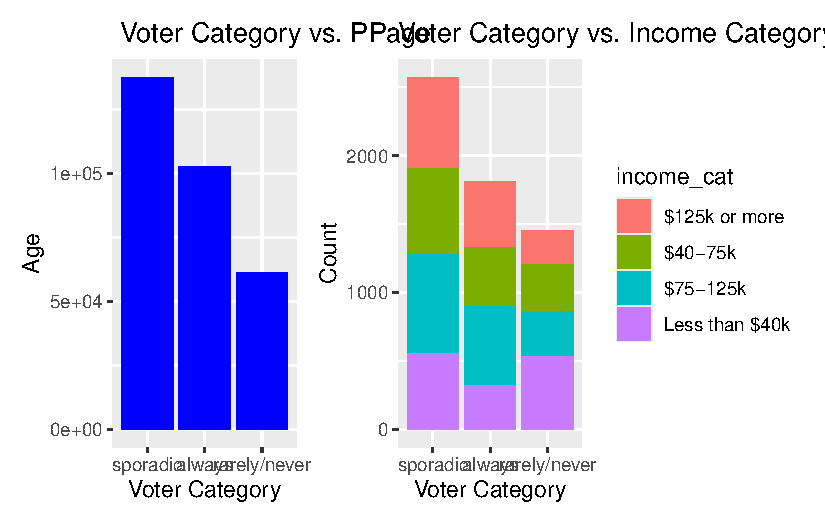
\includegraphics{Lab4_multinom_Questions-1_files/figure-pdf/unnamed-chunk-8-1.pdf}

\begin{itemize}
\tightlist
\item
  Fit a model using mean-centered age, race, gender, income, and
  education to predict voter category. Show the code used to fit the
  model, but do \textbf{not} display the model output.
\end{itemize}

\begin{Shaded}
\begin{Highlighting}[]
   \FunctionTok{library}\NormalTok{(nnet)}
    
    \CommentTok{\#Enter code}
\NormalTok{    model }\OtherTok{\textless{}{-}} \FunctionTok{multinom}\NormalTok{(voter\_category }\SpecialCharTok{\textasciitilde{}}\NormalTok{ ppage\_centered}\SpecialCharTok{+}\NormalTok{race}\SpecialCharTok{+}\NormalTok{gender}\SpecialCharTok{+}\NormalTok{income\_cat}\SpecialCharTok{+}\NormalTok{educ , }\AttributeTok{data =}\NormalTok{ voter\_data) }
\end{Highlighting}
\end{Shaded}

\begin{verbatim}
# weights:  36 (22 variable)
initial  value 6411.501317 
iter  10 value 5787.319553
iter  20 value 5710.106757
final  value 5693.312867 
converged
\end{verbatim}

\begin{Shaded}
\begin{Highlighting}[]
    \FunctionTok{summary}\NormalTok{(model)}
\end{Highlighting}
\end{Shaded}

\begin{verbatim}
Call:
multinom(formula = voter_category ~ ppage_centered + race + gender + 
    income_cat + educ, data = voter_data)

Coefficients:
             (Intercept) ppage_centered raceHispanic raceOther/Mixed raceWhite
always        -0.2930636     0.01302944  -0.41064914      -0.3098896 0.1666330
rarely/never  -1.5717468    -0.04756711   0.00653516       0.3728727 0.1274334
              genderMale income_cat$40-75k income_cat$75-125k
always       -0.11444321        0.06029828       0.1474791658
rarely/never  0.09612722        0.12720614       0.0008327606
             income_catLess than $40k educHigh school or less educSome college
always                    -0.09375046              -0.4307847      -0.05493845
rarely/never               0.66256504               0.9221824       0.35703209

Std. Errors:
             (Intercept) ppage_centered raceHispanic raceOther/Mixed  raceWhite
always         0.1064595    0.001954865    0.1212049       0.1546103 0.08711378
rarely/never   0.1313277    0.002287714    0.1256846       0.1567324 0.10173736
             genderMale income_cat$40-75k income_cat$75-125k
always       0.06270386        0.09207983          0.0842924
rarely/never 0.07068793        0.11021246          0.1059299
             income_catLess than $40k educHigh school or less educSome college
always                      0.1027393              0.08639085       0.07673907
rarely/never                0.1121243              0.09566403       0.09377194

Residual Deviance: 11386.63 
AIC: 11430.63 
\end{verbatim}

\begin{itemize}
\tightlist
\item
  \emph{Should party identification be added to the model?}
\item
  \#Hint: Use an anova test to make the determination
\end{itemize}

\begin{Shaded}
\begin{Highlighting}[]
\CommentTok{\#Enter code}
\NormalTok{    model2 }\OtherTok{\textless{}{-}} \FunctionTok{multinom}\NormalTok{(voter\_category }\SpecialCharTok{\textasciitilde{}}\NormalTok{ ppage\_centered}\SpecialCharTok{+}\NormalTok{race}\SpecialCharTok{+}\NormalTok{gender}\SpecialCharTok{+}\NormalTok{income\_cat}\SpecialCharTok{+}\NormalTok{educ}\SpecialCharTok{+}\NormalTok{pol\_ident\_new , }\AttributeTok{data =}\NormalTok{ voter\_data) }
\end{Highlighting}
\end{Shaded}

\begin{verbatim}
# weights:  45 (28 variable)
initial  value 6411.501317 
iter  10 value 5712.138215
iter  20 value 5630.480535
iter  30 value 5617.781229
final  value 5616.390878 
converged
\end{verbatim}

\begin{Shaded}
\begin{Highlighting}[]
\FunctionTok{summary}\NormalTok{(model2)}
\end{Highlighting}
\end{Shaded}

\begin{verbatim}
Call:
multinom(formula = voter_category ~ ppage_centered + race + gender + 
    income_cat + educ + pol_ident_new, data = voter_data)

Coefficients:
             (Intercept) ppage_centered raceHispanic raceOther/Mixed  raceWhite
always        -0.2411758     0.01252151  -0.38124890      -0.2680365 0.20474650
rarely/never  -1.7315773    -0.04568583  -0.04024104       0.3324263 0.07753584
              genderMale income_cat$40-75k income_cat$75-125k
always       -0.10212938        0.07337959         0.15268950
rarely/never  0.09005921        0.07376215        -0.01249317
             income_catLess than $40k educHigh school or less educSome college
always                    -0.07629406              -0.4139089      -0.03742667
rarely/never               0.58781862               0.8532964       0.29289159
             pol_ident_newIndep pol_ident_newOther pol_ident_newRep
always               -0.1698740         -0.4605512      -0.07796573
rarely/never          0.3924389          0.9404568       0.08381229

Std. Errors:
             (Intercept) ppage_centered raceHispanic raceOther/Mixed  raceWhite
always         0.1078881    0.001964019    0.1222822       0.1560996 0.09266425
rarely/never   0.1360832    0.002324481    0.1280062       0.1590606 0.10784955
             genderMale income_cat$40-75k income_cat$75-125k
always       0.06322716        0.09227759         0.08441574
rarely/never 0.07217159        0.11136556         0.10662568
             income_catLess than $40k educHigh school or less educSome college
always                      0.1030657              0.08698980       0.07734979
rarely/never                0.1137400              0.09739894       0.09520346
             pol_ident_newIndep pol_ident_newOther pol_ident_newRep
always               0.08404605          0.1211546       0.08191505
rarely/never         0.09769631          0.1062289       0.10276761

Residual Deviance: 11232.78 
AIC: 11288.78 
\end{verbatim}

\begin{Shaded}
\begin{Highlighting}[]
\FunctionTok{anova}\NormalTok{(model,model2)}
\end{Highlighting}
\end{Shaded}

\begin{verbatim}
                                                               Model Resid. df
1                 ppage_centered + race + gender + income_cat + educ     11650
2 ppage_centered + race + gender + income_cat + educ + pol_ident_new     11644
  Resid. Dev   Test    Df LR stat. Pr(Chi)
1   11386.63           NA       NA      NA
2   11232.78 1 vs 2     6  153.844       0
\end{verbatim}

\begin{verbatim}
> #Enter answer based on your code: Yes! There is significant gain in variance explained
\end{verbatim}

\textbf{Use the model you select for the remainder of the assignment}.

\subsection{LRT}\label{lrt}

\begin{itemize}
\item
  Run the full model and report overall significance of each of the
  terms

\begin{Shaded}
\begin{Highlighting}[]
\FunctionTok{Anova}\NormalTok{(model2)}
\end{Highlighting}
\end{Shaded}

\begin{verbatim}
Analysis of Deviance Table (Type II tests)

Response: voter_category
               LR Chisq Df Pr(>Chisq)    
ppage_centered   638.30  2  < 2.2e-16 ***
race              52.65  6  1.379e-09 ***
gender             6.03  2     0.0491 *  
income_cat        67.72  6  1.198e-12 ***
educ             154.14  4  < 2.2e-16 ***
pol_ident_new    153.84  6  < 2.2e-16 ***
---
Signif. codes:  0 '***' 0.001 '**' 0.01 '*' 0.05 '.' 0.1 ' ' 1
\end{verbatim}
\end{itemize}

\subsection{Marginal Effects Political Group -
Emmeans}\label{marginal-effects-political-group---emmeans}

\begin{Shaded}
\begin{Highlighting}[]
\CommentTok{\#Get estimated marginal means from the model}

\CommentTok{\#using }
\NormalTok{multinomial\_analysis\_age }\OtherTok{\textless{}{-}} \FunctionTok{emmeans}\NormalTok{(model2, }\SpecialCharTok{\textasciitilde{}}\NormalTok{ pol\_ident\_new}\SpecialCharTok{|}\NormalTok{voter\_category)}


\NormalTok{coefs }\OtherTok{=} \FunctionTok{contrast}\NormalTok{(}\FunctionTok{regrid}\NormalTok{(multinomial\_analysis\_age, }\StringTok{"log"}\NormalTok{),}\StringTok{"trt.vs.ctrl1"}\NormalTok{,  }\AttributeTok{by=}\StringTok{"pol\_ident\_new"}\NormalTok{)}
\CommentTok{\# you can add a parameter to the above command, ref = newbaseline, if you want to change baseline}

\FunctionTok{update}\NormalTok{(coefs, }\AttributeTok{by =} \StringTok{"contrast"}\NormalTok{) }\SpecialCharTok{\%\textgreater{}\%} 
  \FunctionTok{kable}\NormalTok{(}\AttributeTok{format =} \StringTok{"markdown"}\NormalTok{, }\AttributeTok{digits =} \DecValTok{3}\NormalTok{)}
\end{Highlighting}
\end{Shaded}

\begin{longtable}[]{@{}
  >{\raggedright\arraybackslash}p{(\columnwidth - 12\tabcolsep) * \real{0.3514}}
  >{\raggedright\arraybackslash}p{(\columnwidth - 12\tabcolsep) * \real{0.1892}}
  >{\raggedleft\arraybackslash}p{(\columnwidth - 12\tabcolsep) * \real{0.1216}}
  >{\raggedleft\arraybackslash}p{(\columnwidth - 12\tabcolsep) * \real{0.0811}}
  >{\raggedleft\arraybackslash}p{(\columnwidth - 12\tabcolsep) * \real{0.0405}}
  >{\raggedleft\arraybackslash}p{(\columnwidth - 12\tabcolsep) * \real{0.1081}}
  >{\raggedleft\arraybackslash}p{(\columnwidth - 12\tabcolsep) * \real{0.1081}}@{}}
\toprule\noalign{}
\begin{minipage}[b]{\linewidth}\raggedright
contrast
\end{minipage} & \begin{minipage}[b]{\linewidth}\raggedright
pol\_ident\_new
\end{minipage} & \begin{minipage}[b]{\linewidth}\raggedleft
estimate
\end{minipage} & \begin{minipage}[b]{\linewidth}\raggedleft
SE
\end{minipage} & \begin{minipage}[b]{\linewidth}\raggedleft
df
\end{minipage} & \begin{minipage}[b]{\linewidth}\raggedleft
t.ratio
\end{minipage} & \begin{minipage}[b]{\linewidth}\raggedleft
p.value
\end{minipage} \\
\midrule\noalign{}
\endhead
\bottomrule\noalign{}
\endlastfoot
always - sporadic & Dem & -0.482 & 0.057 & 28 & -8.478 & 0.000 \\
(rarely/never) - sporadic & Dem & -0.961 & 0.070 & 28 & -13.722 &
0.000 \\
always - sporadic & Indep & -0.640 & 0.072 & 28 & -8.954 & 0.000 \\
(rarely/never) - sporadic & Indep & -0.591 & 0.077 & 28 & -7.643 &
0.000 \\
always - sporadic & Other & -0.913 & 0.111 & 28 & -8.263 & 0.000 \\
(rarely/never) - sporadic & Other & -0.078 & 0.087 & 28 & -0.902 &
0.747 \\
always - sporadic & Rep & -0.556 & 0.071 & 28 & -7.885 & 0.000 \\
(rarely/never) - sporadic & Rep & -0.883 & 0.084 & 28 & -10.469 &
0.000 \\
\end{longtable}

\subsection{Marginal Effects of Education -
Emmeans}\label{marginal-effects-of-education---emmeans}

\begin{Shaded}
\begin{Highlighting}[]
\CommentTok{\#Enter code}
\NormalTok{multinomial\_analysis\_educ }\OtherTok{\textless{}{-}} \FunctionTok{emmeans}\NormalTok{(model2, }\SpecialCharTok{\textasciitilde{}}\NormalTok{ educ}\SpecialCharTok{|}\NormalTok{voter\_category)}

\NormalTok{coefs }\OtherTok{=} \FunctionTok{contrast}\NormalTok{(}\FunctionTok{regrid}\NormalTok{(multinomial\_analysis\_educ, }\StringTok{"log"}\NormalTok{),}\StringTok{"trt.vs.ctrl1"}\NormalTok{,  }\AttributeTok{by=}\StringTok{"educ"}\NormalTok{)}
\CommentTok{\# you can add a parameter to the above command, ref = newbaseline, if you want to change baseline}

\FunctionTok{update}\NormalTok{(coefs, }\AttributeTok{by =} \StringTok{"contrast"}\NormalTok{) }\SpecialCharTok{\%\textgreater{}\%} 
  \FunctionTok{kable}\NormalTok{(}\AttributeTok{format =} \StringTok{"markdown"}\NormalTok{, }\AttributeTok{digits =} \DecValTok{3}\NormalTok{)}
\end{Highlighting}
\end{Shaded}

\begin{longtable}[]{@{}
  >{\raggedright\arraybackslash}p{(\columnwidth - 12\tabcolsep) * \real{0.3250}}
  >{\raggedright\arraybackslash}p{(\columnwidth - 12\tabcolsep) * \real{0.2500}}
  >{\raggedleft\arraybackslash}p{(\columnwidth - 12\tabcolsep) * \real{0.1125}}
  >{\raggedleft\arraybackslash}p{(\columnwidth - 12\tabcolsep) * \real{0.0750}}
  >{\raggedleft\arraybackslash}p{(\columnwidth - 12\tabcolsep) * \real{0.0375}}
  >{\raggedleft\arraybackslash}p{(\columnwidth - 12\tabcolsep) * \real{0.1000}}
  >{\raggedleft\arraybackslash}p{(\columnwidth - 12\tabcolsep) * \real{0.1000}}@{}}
\toprule\noalign{}
\begin{minipage}[b]{\linewidth}\raggedright
contrast
\end{minipage} & \begin{minipage}[b]{\linewidth}\raggedright
educ
\end{minipage} & \begin{minipage}[b]{\linewidth}\raggedleft
estimate
\end{minipage} & \begin{minipage}[b]{\linewidth}\raggedleft
SE
\end{minipage} & \begin{minipage}[b]{\linewidth}\raggedleft
df
\end{minipage} & \begin{minipage}[b]{\linewidth}\raggedleft
t.ratio
\end{minipage} & \begin{minipage}[b]{\linewidth}\raggedleft
p.value
\end{minipage} \\
\midrule\noalign{}
\endhead
\bottomrule\noalign{}
\endlastfoot
always - sporadic & College & -0.509 & 0.060 & 28 & -8.497 & 0.000 \\
(rarely/never) - sporadic & College & -0.986 & 0.076 & 28 & -12.904 &
0.000 \\
always - sporadic & High school or less & -0.898 & 0.074 & 28 & -12.189
& 0.000 \\
(rarely/never) - sporadic & High school or less & -0.187 & 0.069 & 28 &
-2.705 & 0.031 \\
always - sporadic & Some college & -0.540 & 0.065 & 28 & -8.357 &
0.000 \\
(rarely/never) - sporadic & Some college & -0.707 & 0.074 & 28 & -9.512
& 0.000 \\
\end{longtable}

\begin{itemize}
\item
  Next, plot the predicted probabilities of voter category as a function
  of Age and Party ID

\begin{Shaded}
\begin{Highlighting}[]
  \FunctionTok{ggemmeans}\NormalTok{(model2, }\AttributeTok{terms =} \FunctionTok{c}\NormalTok{(}\StringTok{"ppage\_centered"}\NormalTok{)) }\SpecialCharTok{\%\textgreater{}\%} 
  \FunctionTok{ggplot}\NormalTok{(., }\FunctionTok{aes}\NormalTok{(}\AttributeTok{x =}\NormalTok{ x, }\AttributeTok{y =}\NormalTok{ predicted , }\AttributeTok{fill =}\NormalTok{ response.level)) }\SpecialCharTok{+}
  \FunctionTok{geom\_area}\NormalTok{() }\SpecialCharTok{+} 
  \FunctionTok{geom\_rug}\NormalTok{(}\AttributeTok{sides =} \StringTok{"b"}\NormalTok{, }\AttributeTok{position =} \StringTok{"jitter"}\NormalTok{, }\AttributeTok{alpha =}\NormalTok{ .}\DecValTok{5}\NormalTok{) }\SpecialCharTok{+} 
  \FunctionTok{labs}\NormalTok{(}\AttributeTok{x =} \StringTok{"}\SpecialCharTok{\textbackslash{}n}\StringTok{Age"}\NormalTok{, }\AttributeTok{y =} \StringTok{"Predicted Probablity}\SpecialCharTok{\textbackslash{}n}\StringTok{"}\NormalTok{, }\AttributeTok{title =} \StringTok{"Predicted Probabilities of Voting Frequency by Age"}\NormalTok{) }\SpecialCharTok{+}
  \FunctionTok{scale\_fill\_manual}\NormalTok{(}
    \AttributeTok{name =} \ConstantTok{NULL}\NormalTok{,}
    \AttributeTok{values =} \FunctionTok{c}\NormalTok{(}\StringTok{"always"} \OtherTok{=} \StringTok{"\#F6B533"}\NormalTok{, }\StringTok{"sporadic"} \OtherTok{=} \StringTok{"\#D07EA2"}\NormalTok{, }\StringTok{"rarely/never"} \OtherTok{=} \StringTok{"\#9854F7"}\NormalTok{),}
    \AttributeTok{labels =} \FunctionTok{c}\NormalTok{(}\StringTok{"RARELY OR NEVER VOTE    "}\NormalTok{, }\StringTok{"SOMETIMES VOTE    "}\NormalTok{, }\StringTok{"ALMOST ALWAYS VOTE    "}\NormalTok{),}
    \AttributeTok{breaks =} \FunctionTok{c}\NormalTok{(}\StringTok{"rarely/never"}\NormalTok{, }\StringTok{"sporadic"}\NormalTok{, }\StringTok{"always"}\NormalTok{)}
\NormalTok{  ) }\SpecialCharTok{+}
  \FunctionTok{theme\_minimal}\NormalTok{()}
\end{Highlighting}
\end{Shaded}

  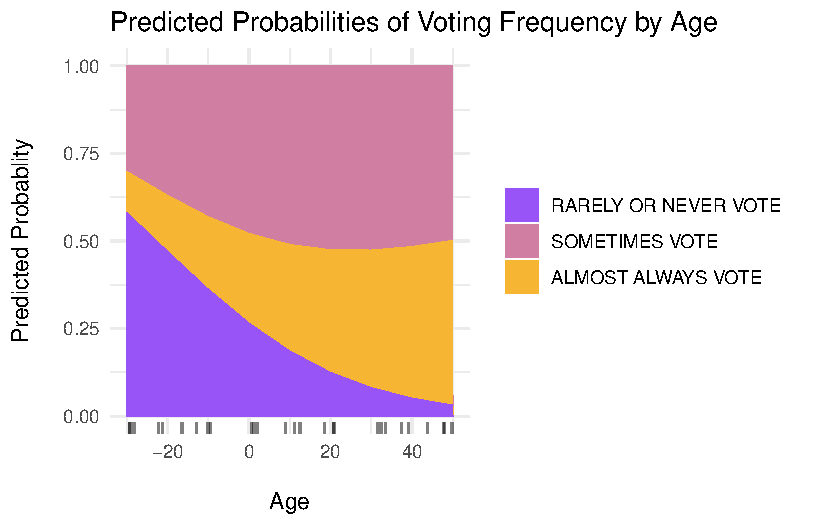
\includegraphics{Lab4_multinom_Questions-1_files/figure-pdf/unnamed-chunk-14-1.pdf}
\end{itemize}

Plot predicted probabilities as a function of education and voting
frequency.

\begin{Shaded}
\begin{Highlighting}[]
\FunctionTok{ggemmeans}\NormalTok{(model2, }\AttributeTok{terms=}\FunctionTok{c}\NormalTok{(}\StringTok{"pol\_ident\_new"}\NormalTok{)) }\SpecialCharTok{\%\textgreater{}\%}
  \FunctionTok{ggplot}\NormalTok{(}\FunctionTok{aes}\NormalTok{(}\AttributeTok{x =}\NormalTok{ x, }\AttributeTok{y =}\NormalTok{ predicted, }\AttributeTok{fill =}\NormalTok{ response.level))}\SpecialCharTok{+}
  \FunctionTok{geom\_bar}\NormalTok{(}\AttributeTok{stat =} \StringTok{"identity"}\NormalTok{ ) }\SpecialCharTok{+} 
   \FunctionTok{geom\_text}\NormalTok{(}\FunctionTok{aes}\NormalTok{(}\AttributeTok{label =} \FunctionTok{round}\NormalTok{(predicted, }\DecValTok{3}\NormalTok{)), }\AttributeTok{color=}\StringTok{"white"}\NormalTok{, }\AttributeTok{position =} \FunctionTok{position\_fill}\NormalTok{(}\AttributeTok{vjust =} \FloatTok{0.5}\NormalTok{),}\AttributeTok{size=}\DecValTok{5}\NormalTok{) }\SpecialCharTok{+} 
  \FunctionTok{labs}\NormalTok{(}\AttributeTok{x=}\StringTok{"polID"}\NormalTok{, }\StringTok{"Predicted Probablity"}\NormalTok{) }\SpecialCharTok{+} 
  \FunctionTok{scale\_fill\_viridis}\NormalTok{(}\AttributeTok{discrete =} \ConstantTok{TRUE}\NormalTok{)}
\end{Highlighting}
\end{Shaded}

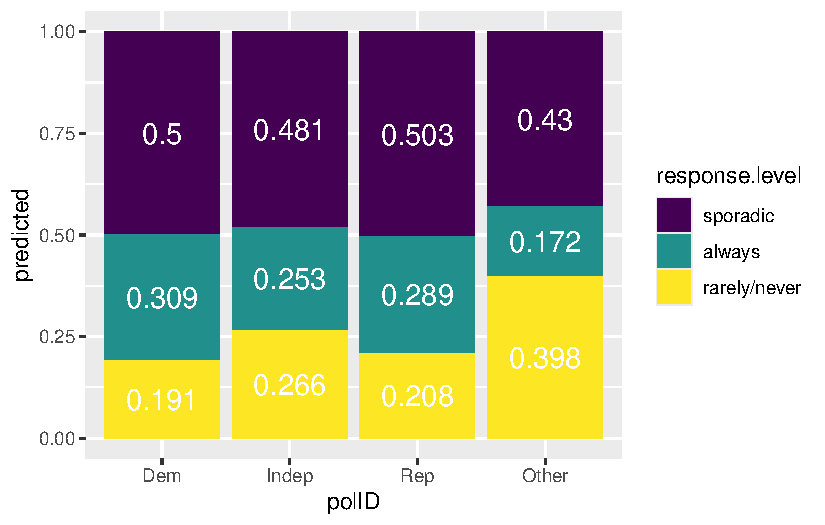
\includegraphics{Lab4_multinom_Questions-1_files/figure-pdf/unnamed-chunk-15-1.pdf}

\begin{Shaded}
\begin{Highlighting}[]
\FunctionTok{ggemmeans}\NormalTok{(model2, }\AttributeTok{terms=}\FunctionTok{c}\NormalTok{(}\StringTok{"educ"}\NormalTok{)) }\SpecialCharTok{\%\textgreater{}\%}
  \FunctionTok{ggplot}\NormalTok{(}\FunctionTok{aes}\NormalTok{(}\AttributeTok{x =}\NormalTok{ x, }\AttributeTok{y =}\NormalTok{ predicted, }\AttributeTok{fill =}\NormalTok{ response.level))}\SpecialCharTok{+}
  \FunctionTok{geom\_bar}\NormalTok{(}\AttributeTok{stat =} \StringTok{"identity"}\NormalTok{ ) }\SpecialCharTok{+} 
   \FunctionTok{geom\_text}\NormalTok{(}\FunctionTok{aes}\NormalTok{(}\AttributeTok{label =} \FunctionTok{round}\NormalTok{(predicted, }\DecValTok{3}\NormalTok{)), }\AttributeTok{color=}\StringTok{"white"}\NormalTok{, }\AttributeTok{position =} \FunctionTok{position\_fill}\NormalTok{(}\AttributeTok{vjust =} \FloatTok{0.5}\NormalTok{),}\AttributeTok{size=}\DecValTok{5}\NormalTok{) }\SpecialCharTok{+} 
  \FunctionTok{labs}\NormalTok{(}\AttributeTok{x=}\StringTok{"Education"}\NormalTok{, }\StringTok{"Predicted Probablity"}\NormalTok{) }\SpecialCharTok{+} 
  \FunctionTok{scale\_fill\_viridis}\NormalTok{(}\AttributeTok{discrete =} \ConstantTok{TRUE}\NormalTok{)}
\end{Highlighting}
\end{Shaded}

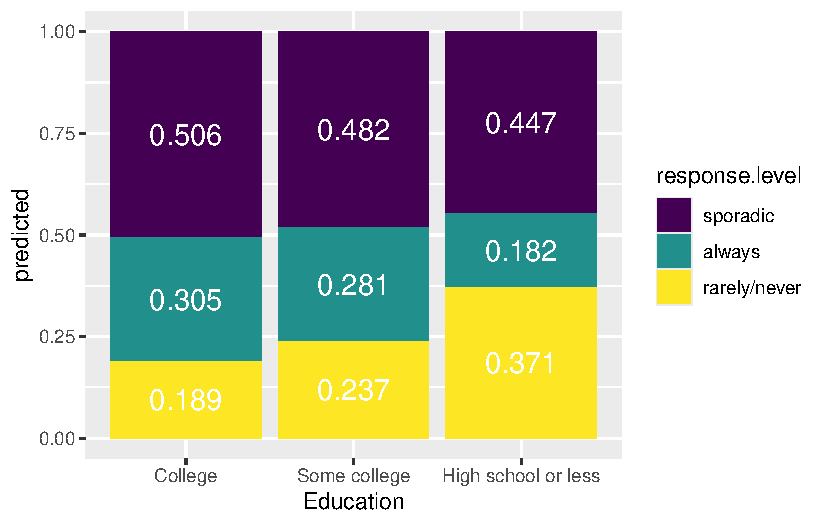
\includegraphics{Lab4_multinom_Questions-1_files/figure-pdf/unnamed-chunk-16-1.pdf}

\subsection{Write-up}\label{write-up}

\subsubsection{Differences between political groups and voting behavior
-
Emmeans}\label{differences-between-political-groups-and-voting-behavior---emmeans}

\begin{Shaded}
\begin{Highlighting}[]
\NormalTok{multi\_an }\OtherTok{\textless{}{-}} \FunctionTok{emmeans}\NormalTok{(model2, }\SpecialCharTok{\textasciitilde{}}\NormalTok{ pol\_ident\_new}\SpecialCharTok{|}\NormalTok{voter\_category)}

\NormalTok{coefs }\OtherTok{=} \FunctionTok{contrast}\NormalTok{(}\FunctionTok{regrid}\NormalTok{(multi\_an, }\StringTok{"log"}\NormalTok{),}\StringTok{"trt.vs.ctrl1"}\NormalTok{,  }\AttributeTok{by=}\StringTok{"pol\_ident\_new"}\NormalTok{)}

\FunctionTok{update}\NormalTok{(coefs, }\AttributeTok{by =} \StringTok{"contrast"}\NormalTok{) }\SpecialCharTok{\%\textgreater{}\%} 
  \FunctionTok{kable}\NormalTok{(}\AttributeTok{format =} \StringTok{"markdown"}\NormalTok{, }\AttributeTok{digits =} \DecValTok{3}\NormalTok{)}
\end{Highlighting}
\end{Shaded}

\begin{longtable}[]{@{}
  >{\raggedright\arraybackslash}p{(\columnwidth - 12\tabcolsep) * \real{0.3514}}
  >{\raggedright\arraybackslash}p{(\columnwidth - 12\tabcolsep) * \real{0.1892}}
  >{\raggedleft\arraybackslash}p{(\columnwidth - 12\tabcolsep) * \real{0.1216}}
  >{\raggedleft\arraybackslash}p{(\columnwidth - 12\tabcolsep) * \real{0.0811}}
  >{\raggedleft\arraybackslash}p{(\columnwidth - 12\tabcolsep) * \real{0.0405}}
  >{\raggedleft\arraybackslash}p{(\columnwidth - 12\tabcolsep) * \real{0.1081}}
  >{\raggedleft\arraybackslash}p{(\columnwidth - 12\tabcolsep) * \real{0.1081}}@{}}
\toprule\noalign{}
\begin{minipage}[b]{\linewidth}\raggedright
contrast
\end{minipage} & \begin{minipage}[b]{\linewidth}\raggedright
pol\_ident\_new
\end{minipage} & \begin{minipage}[b]{\linewidth}\raggedleft
estimate
\end{minipage} & \begin{minipage}[b]{\linewidth}\raggedleft
SE
\end{minipage} & \begin{minipage}[b]{\linewidth}\raggedleft
df
\end{minipage} & \begin{minipage}[b]{\linewidth}\raggedleft
t.ratio
\end{minipage} & \begin{minipage}[b]{\linewidth}\raggedleft
p.value
\end{minipage} \\
\midrule\noalign{}
\endhead
\bottomrule\noalign{}
\endlastfoot
always - sporadic & Dem & -0.482 & 0.057 & 28 & -8.478 & 0.000 \\
(rarely/never) - sporadic & Dem & -0.961 & 0.070 & 28 & -13.722 &
0.000 \\
always - sporadic & Indep & -0.640 & 0.072 & 28 & -8.954 & 0.000 \\
(rarely/never) - sporadic & Indep & -0.591 & 0.077 & 28 & -7.643 &
0.000 \\
always - sporadic & Other & -0.913 & 0.111 & 28 & -8.263 & 0.000 \\
(rarely/never) - sporadic & Other & -0.078 & 0.087 & 28 & -0.902 &
0.747 \\
always - sporadic & Rep & -0.556 & 0.071 & 28 & -7.885 & 0.000 \\
(rarely/never) - sporadic & Rep & -0.883 & 0.084 & 28 & -10.469 &
0.000 \\
\end{longtable}

\begin{Shaded}
\begin{Highlighting}[]
\CommentTok{\# get difference between yes{-}no and fair{-}excellent}
\FunctionTok{contrast}\NormalTok{(coefs, }\StringTok{"revpairwise"}\NormalTok{, }\AttributeTok{by =} \StringTok{"contrast"}\NormalTok{) }\SpecialCharTok{\%\textgreater{}\%}
  \FunctionTok{kable}\NormalTok{(}\AttributeTok{format =} \StringTok{"markdown"}\NormalTok{, }\AttributeTok{digits =} \DecValTok{3}\NormalTok{)}
\end{Highlighting}
\end{Shaded}

\begin{longtable}[]{@{}
  >{\raggedright\arraybackslash}p{(\columnwidth - 12\tabcolsep) * \real{0.1892}}
  >{\raggedright\arraybackslash}p{(\columnwidth - 12\tabcolsep) * \real{0.3514}}
  >{\raggedleft\arraybackslash}p{(\columnwidth - 12\tabcolsep) * \real{0.1216}}
  >{\raggedleft\arraybackslash}p{(\columnwidth - 12\tabcolsep) * \real{0.0811}}
  >{\raggedleft\arraybackslash}p{(\columnwidth - 12\tabcolsep) * \real{0.0405}}
  >{\raggedleft\arraybackslash}p{(\columnwidth - 12\tabcolsep) * \real{0.1081}}
  >{\raggedleft\arraybackslash}p{(\columnwidth - 12\tabcolsep) * \real{0.1081}}@{}}
\toprule\noalign{}
\begin{minipage}[b]{\linewidth}\raggedright
contrast1
\end{minipage} & \begin{minipage}[b]{\linewidth}\raggedright
contrast
\end{minipage} & \begin{minipage}[b]{\linewidth}\raggedleft
estimate
\end{minipage} & \begin{minipage}[b]{\linewidth}\raggedleft
SE
\end{minipage} & \begin{minipage}[b]{\linewidth}\raggedleft
df
\end{minipage} & \begin{minipage}[b]{\linewidth}\raggedleft
t.ratio
\end{minipage} & \begin{minipage}[b]{\linewidth}\raggedleft
p.value
\end{minipage} \\
\midrule\noalign{}
\endhead
\bottomrule\noalign{}
\endlastfoot
Indep - Dem & always - sporadic & -0.159 & 0.083 & 28 & -1.918 &
0.244 \\
Other - Dem & always - sporadic & -0.432 & 0.120 & 28 & -3.598 &
0.006 \\
Other - Indep & always - sporadic & -0.273 & 0.126 & 28 & -2.171 &
0.156 \\
Rep - Dem & always - sporadic & -0.075 & 0.081 & 28 & -0.927 & 0.791 \\
Rep - Indep & always - sporadic & 0.084 & 0.085 & 28 & 0.989 & 0.757 \\
Rep - Other & always - sporadic & 0.357 & 0.123 & 28 & 2.905 & 0.034 \\
Indep - Dem & (rarely/never) - sporadic & 0.370 & 0.094 & 28 & 3.933 &
0.003 \\
Other - Dem & (rarely/never) - sporadic & 0.883 & 0.103 & 28 & 8.578 &
0.000 \\
Other - Indep & (rarely/never) - sporadic & 0.513 & 0.107 & 28 & 4.807 &
0.000 \\
Rep - Dem & (rarely/never) - sporadic & 0.078 & 0.099 & 28 & 0.787 &
0.860 \\
Rep - Indep & (rarely/never) - sporadic & -0.292 & 0.099 & 28 & -2.965 &
0.029 \\
Rep - Other & (rarely/never) - sporadic & -0.805 & 0.109 & 28 & -7.404 &
0.000 \\
\end{longtable}

\subsubsection{Differences between education level and voting behavior -
Emmeans}\label{differences-between-education-level-and-voting-behavior---emmeans}

Last part of the assignment: Interpret the results from running the
following code for your model

\begin{Shaded}
\begin{Highlighting}[]
\NormalTok{multi\_an }\OtherTok{\textless{}{-}} \FunctionTok{emmeans}\NormalTok{(model2, }\SpecialCharTok{\textasciitilde{}}\NormalTok{ educ}\SpecialCharTok{|}\NormalTok{voter\_category)}

\NormalTok{coefs }\OtherTok{=} \FunctionTok{contrast}\NormalTok{(}\FunctionTok{regrid}\NormalTok{(multi\_an, }\StringTok{"log"}\NormalTok{),}\StringTok{"trt.vs.ctrl1"}\NormalTok{,  }\AttributeTok{by=}\StringTok{"educ"}\NormalTok{)}

\FunctionTok{update}\NormalTok{(coefs, }\AttributeTok{by =} \StringTok{"contrast"}\NormalTok{) }\SpecialCharTok{\%\textgreater{}\%} 
  \FunctionTok{kable}\NormalTok{(}\AttributeTok{format =} \StringTok{"markdown"}\NormalTok{, }\AttributeTok{digits =} \DecValTok{3}\NormalTok{)}
\end{Highlighting}
\end{Shaded}

\begin{longtable}[]{@{}
  >{\raggedright\arraybackslash}p{(\columnwidth - 12\tabcolsep) * \real{0.3250}}
  >{\raggedright\arraybackslash}p{(\columnwidth - 12\tabcolsep) * \real{0.2500}}
  >{\raggedleft\arraybackslash}p{(\columnwidth - 12\tabcolsep) * \real{0.1125}}
  >{\raggedleft\arraybackslash}p{(\columnwidth - 12\tabcolsep) * \real{0.0750}}
  >{\raggedleft\arraybackslash}p{(\columnwidth - 12\tabcolsep) * \real{0.0375}}
  >{\raggedleft\arraybackslash}p{(\columnwidth - 12\tabcolsep) * \real{0.1000}}
  >{\raggedleft\arraybackslash}p{(\columnwidth - 12\tabcolsep) * \real{0.1000}}@{}}
\toprule\noalign{}
\begin{minipage}[b]{\linewidth}\raggedright
contrast
\end{minipage} & \begin{minipage}[b]{\linewidth}\raggedright
educ
\end{minipage} & \begin{minipage}[b]{\linewidth}\raggedleft
estimate
\end{minipage} & \begin{minipage}[b]{\linewidth}\raggedleft
SE
\end{minipage} & \begin{minipage}[b]{\linewidth}\raggedleft
df
\end{minipage} & \begin{minipage}[b]{\linewidth}\raggedleft
t.ratio
\end{minipage} & \begin{minipage}[b]{\linewidth}\raggedleft
p.value
\end{minipage} \\
\midrule\noalign{}
\endhead
\bottomrule\noalign{}
\endlastfoot
always - sporadic & College & -0.509 & 0.060 & 28 & -8.497 & 0.000 \\
(rarely/never) - sporadic & College & -0.986 & 0.076 & 28 & -12.904 &
0.000 \\
always - sporadic & High school or less & -0.898 & 0.074 & 28 & -12.189
& 0.000 \\
(rarely/never) - sporadic & High school or less & -0.187 & 0.069 & 28 &
-2.705 & 0.031 \\
always - sporadic & Some college & -0.540 & 0.065 & 28 & -8.357 &
0.000 \\
(rarely/never) - sporadic & Some college & -0.707 & 0.074 & 28 & -9.512
& 0.000 \\
\end{longtable}

\begin{Shaded}
\begin{Highlighting}[]
\CommentTok{\# get difference between yes{-}no and fair{-}excellent}
\FunctionTok{contrast}\NormalTok{(coefs, }\StringTok{"revpairwise"}\NormalTok{, }\AttributeTok{by =} \StringTok{"contrast"}\NormalTok{) }\SpecialCharTok{\%\textgreater{}\%}
  \FunctionTok{kable}\NormalTok{(}\AttributeTok{format =} \StringTok{"markdown"}\NormalTok{, }\AttributeTok{digits =} \DecValTok{3}\NormalTok{)}
\end{Highlighting}
\end{Shaded}

\begin{longtable}[]{@{}
  >{\raggedright\arraybackslash}p{(\columnwidth - 12\tabcolsep) * \real{0.3684}}
  >{\raggedright\arraybackslash}p{(\columnwidth - 12\tabcolsep) * \real{0.2737}}
  >{\raggedleft\arraybackslash}p{(\columnwidth - 12\tabcolsep) * \real{0.0947}}
  >{\raggedleft\arraybackslash}p{(\columnwidth - 12\tabcolsep) * \real{0.0632}}
  >{\raggedleft\arraybackslash}p{(\columnwidth - 12\tabcolsep) * \real{0.0316}}
  >{\raggedleft\arraybackslash}p{(\columnwidth - 12\tabcolsep) * \real{0.0842}}
  >{\raggedleft\arraybackslash}p{(\columnwidth - 12\tabcolsep) * \real{0.0842}}@{}}
\toprule\noalign{}
\begin{minipage}[b]{\linewidth}\raggedright
contrast1
\end{minipage} & \begin{minipage}[b]{\linewidth}\raggedright
contrast
\end{minipage} & \begin{minipage}[b]{\linewidth}\raggedleft
estimate
\end{minipage} & \begin{minipage}[b]{\linewidth}\raggedleft
SE
\end{minipage} & \begin{minipage}[b]{\linewidth}\raggedleft
df
\end{minipage} & \begin{minipage}[b]{\linewidth}\raggedleft
t.ratio
\end{minipage} & \begin{minipage}[b]{\linewidth}\raggedleft
p.value
\end{minipage} \\
\midrule\noalign{}
\endhead
\bottomrule\noalign{}
\endlastfoot
High school or less - College & always - sporadic & -0.389 & 0.087 & 28
& -4.492 & 0.000 \\
Some college - College & always - sporadic & -0.031 & 0.076 & 28 &
-0.412 & 0.911 \\
Some college - High school or less & always - sporadic & 0.358 & 0.085 &
28 & 4.220 & 0.001 \\
High school or less - College & (rarely/never) - sporadic & 0.799 &
0.095 & 28 & 8.416 & 0.000 \\
Some college - College & (rarely/never) - sporadic & 0.278 & 0.092 & 28
& 3.030 & 0.014 \\
Some college - High school or less & (rarely/never) - sporadic & -0.520
& 0.088 & 28 & -5.920 & 0.000 \\
\end{longtable}

Enter your interpretation here: People with higher education show a
stronger contrast between ``sporadic voters'' vs.~``always'' or
``rarely/never'' voters. As education level goes up, the more frequently
people vote. However, people with college education are less likely to
vote frequently, as compared to sporadically.



\end{document}
